% This LaTeX document needs to be compiled with XeLaTeX.
\documentclass[10pt]{article}
\usepackage{graphicx}
\usepackage[export]{adjustbox}
\graphicspath{ {./images/} }
\usepackage[fallback]{xeCJK}
\usepackage{polyglossia}
\usepackage{fontspec}
\setCJKmainfont{Noto Serif CJK JP}

\setmainlanguage{polish}
\setmainfont{CMU Serif}

\title{LIGA MATEMATYCZNA im. Zdzisława Matuskiego PÓŁFINAモ \\
 11 lutego 2014 \\
 SZKOŁA PODSTAWOWA }

\author{}
\date{}


\begin{document}
\maketitle
\section*{ZADANIE 1.}
Uzupełnij diagram w taki sposób, aby liczba w każdym polu w rzędzie wyższym była sumą dwóch liczb z pól niższego rzędu sąsiadujących z nim. Oblicz sumę liczb w podstawie diagramu.\\
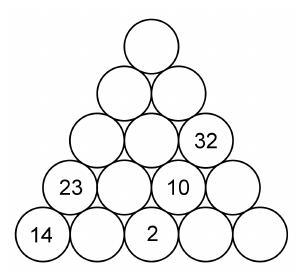
\includegraphics[max width=\textwidth, center]{2024_11_21_cb616dfad60f996777b8g-1}

\section*{ZADANIE 2.}
Krzyś pomnożył trzy liczby naturalne i otrzymał 5400. Liczby pierwsza i druga nie dzielą się przez 2, druga i trzecia - nie dzielą się przez 3, a pierwsza i trzecia - nie dzielą się przez 5. Jakie to liczby?

\section*{ZADANIE 3.}
Suma cyfr pewnej liczby dziewięciocyfrowej jest równa 9. Cyfra 2 występuje w niej tylko raz. Oblicz iloczyn cyfr tej liczby.

\section*{ZADANIE 4.}
O czterech kolegach wiadomo, że:

\begin{itemize}
  \item Mirek i kierowca są starsi od Pawła;
  \item Leszek i policjant trenują boks;
  \item elektryk jest najmłodszy z całej czwórki;
  \item w soboty Zbyszek i piekarz grają w brydża przeciw Pawłowi i elektrykowi.
\end{itemize}

Jaki zawód wykonuje każdy z przyjaciół?

\section*{ZADANIE 5.}
W kredensie stoją 24 dzbany, w tym 8 z nich jest pustych, 11 wypełnionych miodem do połowy, 5 pełnych miodu. W jaki sposób można podzielić miód i dzbany między trzech braci tak, aby każdy z nich otrzymał 8 dzbanów z jednakową zawartością w nich miodu? (Nie wolno przelewać miodu z dzbana do dzbana.)


\end{document}